\section{Hardware laget og konfiguration af periferienheder}
I det kommende afsnit vil den valgt hardware konfiguration gennemgås. 
Den dybere tekniske beskrivelse i forhold til produkt specifikke registre eller anden speciel arkitektur, vil ikke i detaljer beskrives, med mindre det er en vigtig del af argumentationen for valget.
Det komplette hardware modul findes i \emph{hardware.c}.

\subsection{Valg af hardware profil}
For at kunne håndtere de forskellige opsætninger af hardware i udviklingsforløbet af equalizerens software, er der lavet forskellige hardware opsætninger, således at man på en nem måde kan skifte imellem dem.
\\
I \textit{global.h} filen, findes to compiler \textbf{\#define} direktiver til makro definitionerne \textbf{EMP} og \textbf{DAC}.
Sammenhænget mellem profilerne ses i figur \ref{fig:hardware_profiler}. 
Således kan man teste softwaren på EMP printet, med den monterede mikrofon indgang og hovedtelefon udgang, ved at vælge \textbf{EMP} profilen.
Fravælges \textbf{EMP} profilen, skifter softwaren over til at bruge projekt printet.
Her kan der vælges imellem DAC eller PWM som udgangssignal.  
Den tilhørende pin-konfiguration for de valgte hardware profiler kan ses i bilag \ref{bilag:pinmap}.

\subsection{CPU clock frekvens}
\begin{wrapfigure}[20]{r}{5cm}
	\centering
	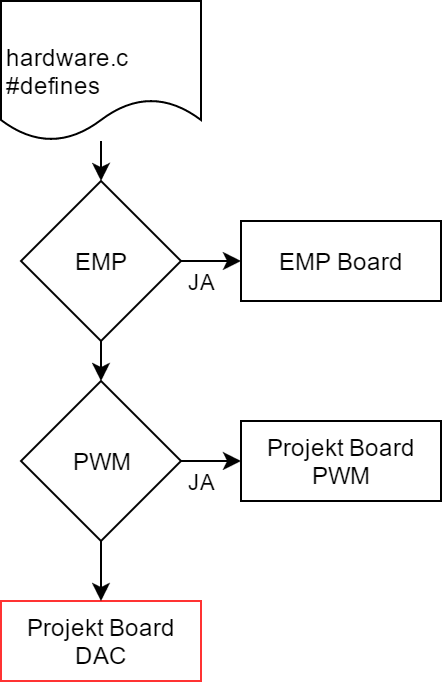
\includegraphics[width=4.5cm]{billeder/hardware_profiles.png}
	\caption{Oversigt over mulige konfigurationer af \textit{hardware.c}.}
	\label{fig:hardware_profiler}
\end{wrapfigure}
For at kunne opnå så mange beregninger som muligt i sekundet, sættes MCU'en clock frekvens til den maksimale.
Den valgte MCU (TM4C123GH6PM) er en $80\si{\mega\hertz}$ mikrokontroller, og den ønskede clock frekvens sættes i funktionen \texttt{set\_80Mhz\_clock()} i hardwaremodulet \textit{hardware.c} til $F_{CPU} = 80\si{\mega\hertz}$. 

Ved denne frekvens kan der på baggrund af den valgte samplefrekvens $F_s$, et mål for hvor mange CPU cycles der er imellem hver sample beregnes til
\begin{align}
N_{CPU cycles} = \frac{F_{CPU}}{F_s}  =  \frac{80\si{\mega\hertz}}{44,1\si{\kilo\hertz}}  = 1814,06 \si{\cycles}
\end{align}

\subsection{ADC}
Til sampling af audiosignalet anvendes en analog til digital konverter (ADC). 
De tre vigtigste faktorer der skal findes frem til er - hvornår bliver der samplet, hvor længe varer det før værdien er tilgængelig og hvor nøjagtig er den samplede værdi.
ADC'en omsætter det analoge lydsignal til en digital repræsentation, i dette tilfælde med en 12 bits opløsning.
Opløsningen på det indgående signal kan bestemmes til $V_{LSb} = (V_{ref+} - V_{ref-} ) / 4096 $, hvor $V_{ref+}$ og $V_{ref-}$ er henholdsvis den positive og negative referencespænding.
I den konkrete løsning, forsynes MCU'en med en single-supply på $V_{DD} = 3,3\si{\volt}$.
Derved bliver den mindste målbare spændingsændring på indgangen

\begin{align}
V_{LSb} = \frac{V_{DD}}{4096} = 8,06\si{\milli\volt\per\LSb}
\end{align}

For et komplet billede af det samplede signal, fremgår det i databladet \cite[afsnit 24.14 s. 1383]{tm4c123gh6pm} for MCU'en, at
den samlede, ikke korrigerede, fejl er $E_T = \pm 30\si{\LSb}$ som maksimum.

Den samplede digitale spænding $V_{d}$, kan således angives med en usikker i forhold til den analoge spænding $V_{a}$ på

\begin{align}
V_{d} = V_{a} \pm \V_{LSb} \cdot E_T = V_{a} \pm   8,06\si{\milli\volt\per\LSb} \cdot 30 \si{\LSb} = V_{a} \pm 24,17\si{\milli\volt}
\end{align} 

Den i projektet anvendte MCU tilbyder en lang række funktionalitet for ADC periferienheden.
Det er dog kun nødvendigt at fortage én sample på hver lyd kanal\footnote{Når software anvedner EMP profil bruges der kun én ADC kanal}, én gang hver sampleperiode $T_s$.
Derfor anvendes en \textbf{Once Mode}, der bliver styret af interrupt service rutinen \textit{sample\_handler()}. Denne ISR og timingen af ADC'en vil bliver uddybet i afsnittet om interrupt.
ADC'ens sampling af indgangssignalet påbegyndes manuelt af equalizerens software.
Samplingen sker ved successiv approksimation (SAR) i ADC'en og ud fra databladet er sampletiden angivet som  $T_C = 2$ ADC clock cycles. 
I implementeringen, er ADC clocken sat til at køre $16 \si{\mega\hertz}$ og giver derved en samplings tid på $T_C = \num{1,25E-7}\si{\second}$.  

\subsection{PWM - Pulse Width Modulation}
I begyndelsen af udviklingen, var der overvejelser om hvordan lydsignalet skulle genskabes efter den digitale behandling var foregået.
Ud fra de indbyggede periferienheder, som den valgte MCU stiller til rådighed, faldt valget på et PWM generet lyd signal.
Det viste sig dog under udviklingen af de analoge filtre, som er gennemgået i foregående kapitel, at opnåelsen af en tilfredsstillende lydkvalitet samt at kunne eftervise equalizerens funktionalitet, ikke kunne opnås med et PWM generet udgangssignal. 
\\

Som udgangspunkt er det anvendte EMP print udstyret med en mikrofonindgang og en hovedtelefonudgang \footnote{Henholdsvis \textbf{Microphone Preamp} og \textbf{Headphone Output} i diagram \cite{emp-diagram}}, som fra designerens udgangspunkt er forbundet med henholds en af MCU'ens analoge indgange og en GPIO pin hvor PWM er mulig.

\begin{figure}[h!]
	\centering
	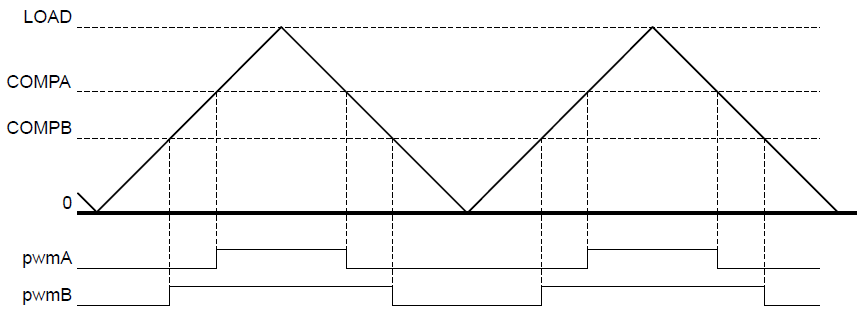
\includegraphics[width=.7\textwidth]{billeder/pwm.png}
	\caption{Eksempel på PWM generator i MCU'en for i fase korrekt modus eller \textbf{Count-Up/Count-down mode}\cite[Fig. 20-5 s. 1232]{tm4c123gh6pm}.}
	\label{fig:pwm}
\end{figure}

Det vælges at bruge PWM i fase korrekte modus, som man kan se et eksempel af i figur \ref{fig:pwm}.
I fase korrekt modus skal PWM tælleren starte på 0 tælle både op til \textbf{LOAD} værdien og ned igen, inden næste PWM cyklus begyndes.
Ved en PWM frekvens $F_{PWM}$ der er den samme som samplingsfrekvensen $F_s$, vil $\textbf{LOAD} = N_{CPU cycles} / 2$.

Da udgangssignalet kan varierer mellem $ 0 \si{\volt}$ og $V_{DD} = 3,3 \si{\volt}$, hvor middelværdien er $V_{DD}/2 = 1,65 \si{\volt}$, kan opløsningen på udgangssignalet beregnes til 

\begin{align}
\Delta V_{PWM} = \frac{V_{DD} \cdot 2K}{N_{CPU cycles}} = \frac{3,3\si{\volt} \cdot 2}{1814} =  3,638\si{\milli\volt}
\end{align}

for et vilkårligt forhold ($K$) imellem samplefrekvens og PWM frekvens. 
Da det er ønskeligt med en PWM frekvens der er 10 gange større end samplingsfrekvensen ($K=10$) ses det, at opløsningen på udgangen ligeledes falder med en faktor 10 til $\Delta V_{PWM} = 36,38\si{\milli\volt}$.\\

Opsætning af PWM findes i \texttt{init\_PWM( INT16U cycles )} i hardware modulet \textit{hardware.c}. Funktionen tager $N_{CPU cycles}$ som parameter, således at hardwaren kan opsættes til andre samplingsfrekvenser end $F_s = 44,1\si{\kilo\hertz}$.
Afhængig af den valgte hardware profil, sættes pin konfigurationen ud fra tabellen i bilag \ref{bilag:pinmap}.  

\FloatBlock

\jj{Mangler overgang til DAC}

\subsection{DAC}
Til at generer udgangssignalet fra MCU'en vælges en ekstern DAC kreds, da MCU'en ikke råder over denne funktionalitet.
Valget blev en \texttt{MCP4922E/P}\footnote{Microchip MCP4922E/P 12-Bit Dual Voltage Output Digital-to-Analog Converter with SPI Interface \cite{mcp4922} } 12bit DAC IC, således at opløsningen på udgangen bliver den samme som på indgangen.
Således er spændingsdifferencen for den mindst betydende bit $ V_{LSb} = V_{ref} / 4096 \approx \num{0,8}\si{\milli\volt} $, ved en ekstern reference spænding på $V_{ref} = 3,3\si{\volt}$.
Derudover har den valgte DAC en maksimal indsvingningstid på $t_{settling} = \num{4.5}\si{\micro\second}$, hvilket passer fint til samplingsperioden på $23\si{\micro\second}$. 

\subsection{SPI}
Den valgte DAC forbindes direkte til MCU'en igennem en SPI bus, de valgte pins er beskrevet i bilag \ref{bilag:pinmap}.
Ifølge databladet er datakommunikation på optil $20\si{\mega\hertz}$ mulig, men SPI port konfigurationen på MCU'en sættes til $10\si{\mega\hertz}$.
For at sætte den ønskede udgangsspænding på DAC'en, er en 16 bit kommando nødvendig. 
I figur \ref{fig:dac12bit_writecmd} ses den nødvendige bitsekvens.
En $10\si{\mega\hertz}$ giver således en kommando overføringstid på $t_{cmd}$ for begge lydkanaler på minimum 
\begin{align}
	t_{cmd} = \frac{N_{kanal} \cdot 16bit}{F_{CLK}} = \frac{2 \cdot 16}{10\si{\mega\hertz}} = 3\si{\micro\second}
\end{align}

\begin{figure}[h!]
	\centering
	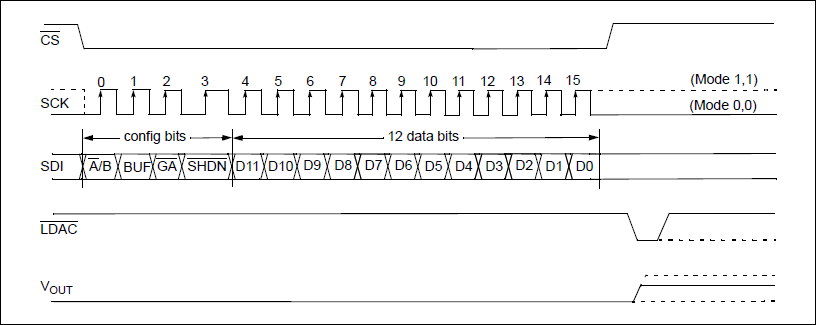
\includegraphics[width=.8\textwidth]{billeder/dac12bit_writecmd.png}
	\caption{Skrive kommando til 12bit MCP4922 DAC.\cite[s. 25]{mcp4922}}
	\label{fig:dac12bit_writecmd}
\end{figure}

I overensstemmelse med databladene for DAC'en og MCU'en, bruges SPI Freescale Fame formatet \footnote{Se afsnit 15.3.4 \cite[s. 954]{tm4c123gh6pm}} i \textbf{Mode 0,0}.

\begin{figure}[h!]
	\centering
	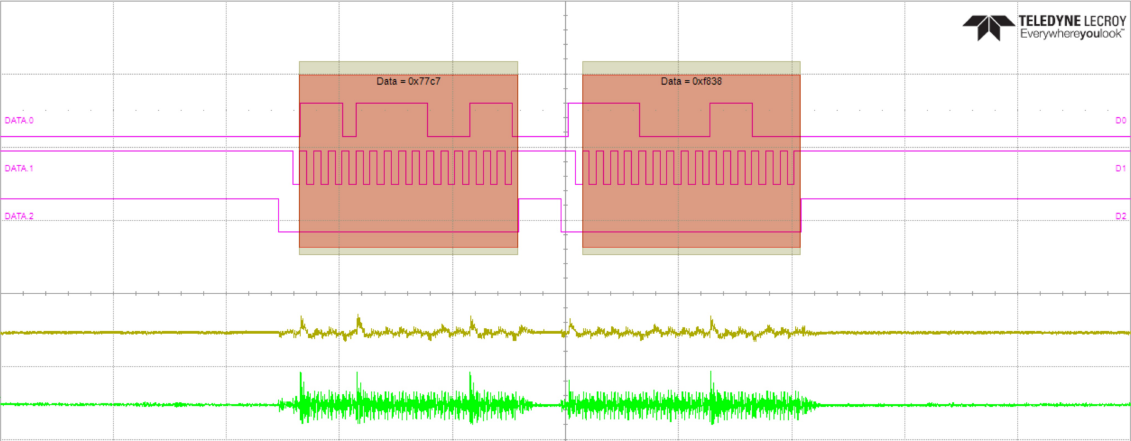
\includegraphics[width=\textwidth]{billeder/dac_dataframe.png}
	\caption{Dataframe til DAC. $1.00\si{\micro\second}\text{/Div}$. \textit{Data.0} = SDI, \textit{Data.1} = SCK, \textit{Data.2} = CS}
	\label{fig:dac_dataframe}
\end{figure}

Konfigurationen af SPI laves i \texttt{spi\_init()} i modulet \textit{hardware.c}  

\FloatBlock

\subsection{Interrupt}
Det er som tidligere fortalt kaldet til \texttt{sample\_handler();} ISR'en der ligger til grund for hele timing af lydsampling med mere.
Det er dog ikke så vigtigt hvilken interrupt vektor der får opgaven.
I dette system er det valgt at bruge \textbf{zero reload event} på PWM'en, som \textit{interrupt trigger}.\\

Konfiguration af \textbf{NVIC}'en kan finde i modulet \textit{tm4c123gh6pm\_startup\_ccs\_gcc.c} og funktionen \texttt{init\_PWM(INT16U cycles);} i hardware modulet \textit{hardware.c}

\subsection{UART}\label{subsec:uart}
Det er muligt at tilgå Shell'en i equalizeren via seriel kommunikation.
I task modellen (figur \ref{fig:eq-taskmodel}) ses kommunikationen mellem \textbf{UART RX/TX} task'ne og Shell tasken.
Grundet hastighedsforskellen imellem scheduleringen af shell'en tasken og den meget langsommere serielle kommunikation, er \textbf{RX/TX queues} implementeret med asymmetrisk størrelse. 
\textbf{TX queue} er således 1KB og \textbf{RX queue} er kun  xx bytes.

Standard opsætningen for seriel kommunikation er
\begin{center}
	\textbf{Baudrate : }19200  \quad \textbf{Databits : } 8 \quad \textbf{Stopbits : }1
\end{center}

Opsætningen af UART'en findes i \texttt{uart0\_init(...);} i uart modulet \textit{uart.c}

\subsection{LCD}
LCD displayet der er monteret på EMP printet, er primært brugt under udvikling til debug information og derfor bliver det brugt på samme måde på projekt printet.
Information som VU-meter, equalizerens tilstand, valgt equalizer profil navn, CPU belastning samt en simpel repræsentation af equalizerens frekvens spektrum kan aflæses på LCD displayet.

LCD modulet er sammensat af et driver API sammen med en \texttt{LCD\_buffer\_task(...);} der sørger for at opdatere selve LCD'en.
Skrivning til LCD displayet sker således ikke direkte
API'et skriver i en shared-memory buffer, som bliver brugt at LCD buffer tasken, se figur \ref{fig:eq-taskmodel}. 
I figur \ref{fig:lcd_task} ses state diagrammet for LCD tasken, hvor \textbf{State N} repræsenterer alle de mellemliggende states.

\begin{figure}[h!]
	\centering
	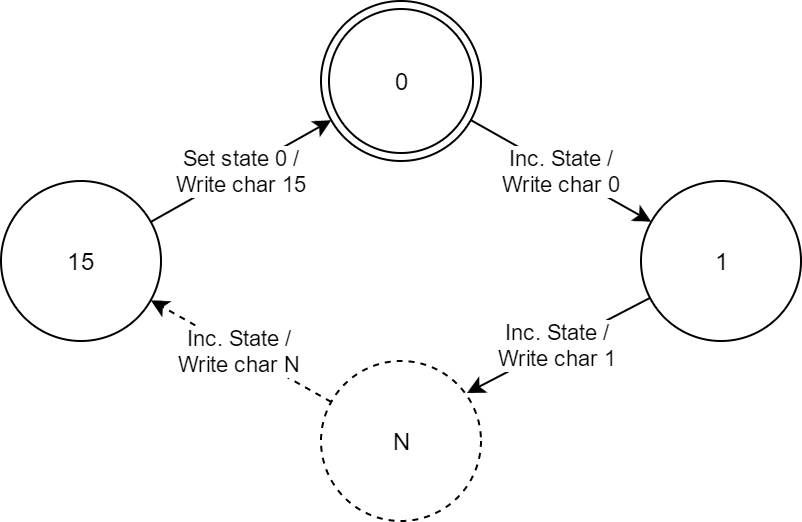
\includegraphics[width=.6\textwidth]{billeder/lcd_task.png}
	\caption{LCD buffer task state diagram.}
	\label{fig:lcd_task}
\end{figure}


LCD displayet bliver initialiseret fra modulet \textit{emp\_lcd1602.c} i  \texttt{lcd\_init();}
  
\FloatBlock

\subsection{Tiva™ C Series TM4C123G LaunchPad Evaluation Board}
Som udviklingsplatform anvendes Tiva LaunchPad \cite{spmu296}. 
Tiva LaunchPad stiller en række funktionalitet til rådighed som fx. On-board ICDI.
Derudover er der på printet også monteret 2 trykkontakter (\textbf{SW1 / SW2}) og en RGB LED, som er medtaget i pin mapping tabellen i bilag \ref{bilag:pinmap}, således at det ikke påvirker hardwareprofilen til projektet.   

\subsection{FPU}
For at kunne gøre brug af FPU'en (floating point unit) på den valgte MCU, kræver denne en produkt specifik aktivering.
Ifølge \cite[afsnit 3.1.5.7 s. 132]{tm4c123gh6pm} er denne implementeret som følger i hardware modulet \textit{hardware.c}.

\lstset{language=C,
	frame=sigle,
	basicstyle=\ttfamily\tiny,
	emph={INT32U,NVIC_CPAC_R},
	emphstyle={\color{blue}},
	keepspaces=true,
	frame=single,
%	numbers=left,
%	numbersep=5pt,
	numberstyle=\tiny\color{black},
	keywordstyle=\color{red}\ttfamily,
	stringstyle=\color{blue}\ttfamily,
	commentstyle=\color{OliveGreen}\ttfamily,
	morecomment=[l][\color{magenta}]{\#}
}
\begin{tabular}{l}
\begin{lstlisting}[title=init\_FPU()]
INT32U reg;
reg = NVIC_CPAC_R;    // Coprocessor Access Control (CPAC) register
reg |= (0xF << 20);   // Set bits 20-23 to enable 
NVIC_CPAC_R = reg;    // 	CP10 and CP11 coprocessors

__asm__("DSB");       // Data Synchronisation Barrier
__asm__("ISB");       // Instruction Synchronisation Barrier
\end{lstlisting}
\end{tabular}

%\subsection{Timers og sysTick}

 